\chapter{Compiler}


Programmiersprachen dienen als Verständigungsmittel zwischen Programmierern und Rechenanlagen. Diese Sprachen haben sich in der Vergangenheit dabei immer mehr an die  Terminologie eines bestimmtes Anwendungsgebietes angenähert. Durch diese Entwicklung eigneten sich Programmiersprachen direkt für die Dokumentation von entwickelten Algorithmen und Anwendungen, entfernten sich jedoch weiter von den Gegebenheiten des realen Rechners.\footcite[Vgl.][S. 15]{Schneider1975}
\begin{figure}[h]
 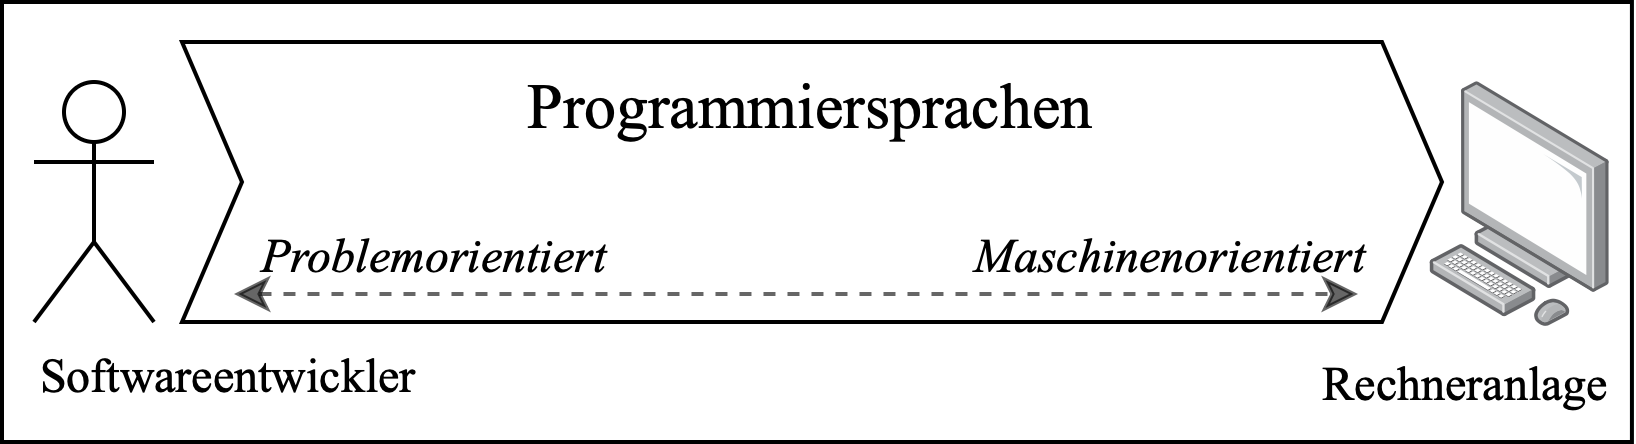
\includegraphics[width=\textwidth,height=\textheight,keepaspectratio]{Images/LanguageIntermediary.png}
 \caption{Programmiersprachen als Schnittstelle}
 \label{fig:Programmiersprachen als Schnittstelle}
\end{figure}
Für die Ausführung einer in einer problemorientierten Programmiersprache geschriebenen Anwendung ist es notwendig, die Sprache in eine maschinenorientierte Form zu überführen. \footcite[Vgl.][S. 15]{Schneider1975} Bereits im Jahre 1951 stelle Rutishauser fest,  dass Computer in der Lage sind diesen Übersetzungsvorgang selbst durchzuführen.\footcite[Vgl.][S. 1]{Quelle fehlt! improve https://link.springer.com/article/10.1007/BF02009622}  %Hier fehlt die Quelle!
\\
Durch die Möglichkeit zur automatischen Übersetzung von problemorientierten Programmiersprachen konnten Hochsprachen entwickelt werden, die menschenfreundliche Sprachelemente anstatt Maschineninstruktionen verwenden. \footcite[Vgl.][S. 47]{Wagenknecht2014}
\section{ Grundbegriffe}

Diese historische Einführung zeigt,  dass Software zur automatisierten Übersetzung schon seit der Mitte des letzten Jahrhunderts thematisiert wurde, so hat sich in der Wissenschaft eine einheitliche Definition ergeben.  \citeauthor{Ullmann2008} beschreibt die sogenannten Compiler im Jahre \citeyear{Ullmann2008} wie folgt:\footcite[Vgl.][S. 1]{Ullmann2008} 
\begin{Def}[Compiler]
Ein Compiler ist ein Programm, welches ein anderes Programm aus einer Quellsprache in ein gleichwertiges Programm einer Zielsprache übersetzen kann.
\end{Def} Aus dieser Definition lässt sich ein für diese Arbeit relevanter Fakt ableiten: Compiler sind nicht ausschließlich Übersetzer zwischen zwischen problemorientierten,- und maschinenorientierten Programmiersprachen.  Sie sind ausschließlich für die Übersetzung von einer Quellsprache in eine Zielsprache verantwortlich.  Die einzige Bedingung ist,  dass die Programme gleichwertig sind.  Darauf basierend haben sich einige Anwendungsfälle für Compiler entwickelt,  die ein anderes Ziel verfolgen. Dazu gehöre zum Beispiel: \footcite[Vgl.][S. 27]{Ullmann2008}\\
\begin{itemize}
\item Binärübersetzung: Dabei wird der Binärcode eines Programmes für einen Rechner in den für einen anderen Rechner übersetzt, sodass er das Computerprogramm Ausführung kann.
\item Interpreter für Datenbankabfragen: Sprachen werden nicht nur für Software eingesetzt sondern auch für Abfragesprachen wie SQL (Structured Query Language).  Diese Datenbankabfragen können zu Befehlen kompiliert werden um in einer Datenbank nach Datensätzen zu suchen. 
\end{itemize}

Ein Source-to-Source(S2S) Compiler , häufig auch als "Transpiler" bezeichnet, ist ebenfalls eine besondere Ausprägung eines Compilers die sich wie folgt definieren lässt.  \footcite[Vgl.][S. 1629]{IJCSIT2015}
\begin{Def}[Source-to-Source Compiler]
Ein Source-to-Source-Compiler ist ein Compiler, bei dem sowohl die Quellsprache als auch die Zielsprache eine Hochsprache ist.
\end{Def}



\subsection{Programm}
Um zu verstehen, wann Programme gleichwertig sind ist es zuerst notwendig ein einheitliches Begriffsverständnis herzustellen.  Auch wenn der Begriff Programm für jedermann geläufig ist,  unterscheidet man in der Literatur die Repräsentationen in denen ein Programm vorkommen kann.
\begin{itemize}
\item Der Quelltext:
\item Ein Objektmodul:
\item Ein ausführbares Programm:
\item Ein Prozess:
\end{itemize}

\subsection{ Syntax und Semantik}
Die Syntax einer Programmiersprache ist das Aussehen bzw. die Struktur des Quelltextes. Der komplette Quelltext eines Programms muss syntaktisch korrekt sein, damit er übersetzt werden kann.  \\
Die Semantik ist die Bedeutung, die den verschiedenen syntaktischen Strukturen zugeordnet werden kann. Es ist also von der Semantik abhängig auf welche Art und Weise die Weiterverabeitung durch den Compiler erfolgt. 




\section{Aufgabe}
Die Aufgaben des Compilers lassen sich, mit dem Ziel der Übersetzung von Programmiersprachen, in die zwei Unteraufgaben Analyse und Synthese unterteilen. \footcite[Vgl.][S. 6]{Ullmann2008}\\
Bei der Analyse wird das Programm in seine Bestandteile zerlegt und mit einer grammatischen Struktur versehen. Diese wird anschließend verwendet um eine Zwischendarstellung des Quellprogramms zu erstellen. Dabei wird überprüft, ob das Programm syntaktisch oder semantisch nicht wohlgeformt ist, und ob der Programmierer Änderungen vornehmen muss. Außerdem werden bei der Analyse Informationen über das Quellprogramm gesammelt und in einer so genannten Symboltabelle abgelegt.  \footcite[Vgl.][S. 6f]{Ullmann2008}\\
Bei der Synthese wird aus der Zwischendarstellung un den Informationen aus der Symboltabelle das gewünschte Zielprogramm konstruiert. Der Teil des Compilers, der sich mit der Analyse befasst wird oft als Front-End bezeichnet, derjenige der für die Synthese zustädnig ist als Back-End.  \footcite[Vgl.][S. 7]{Ullmann2008}
\section{Phasen}
Der Vorgang des Kompilieren lässt sich nach \citeauthor{Ullmann2008} in mehere Phasen unterteilen, die an dieser Stelle eingeführt werden sollen. \footcite[Vgl.][S. 6]{Ullmann2008}
\subsection{Lexikalische Analyse}
Die erste Phase eines Compilers ist die sogenannte lexikalische Analyse. Dabei wird der Zeichenstream, der das Quellprogramm bildet in Lexeme gegliedert. Für jedes erzeugte Lexem gibt der lexikalische analysator ein Token in folgender Form aus:\footcite[Vgl.][S. 7f]{Ullmann2008}
\begin{center}
 <Name, Attributwert>
\end{center}
Der Name ist dabei ein abstaktes Symbol, das während der nächste Phase, der Syntaxanalyse verwendet wird. Der Attributwert auf einen Eintrag in der symboltabelle für dieses Token zeigt. Diese Informationen werden in den späteren Phasen für die semantische Analyse und die Codegeneriung benötigt. \footcite[Vgl.][S. 7f]{Ullmann2008}
\subsection{Syntaxanalyse}
Die zweite Phase des Compilers ist die Syntaxanalye. Dafür verwendet der sogenannte Parser die vom lexikalischen Analysator ausgegebenen Token um eine baumartige Zwischendarstellung zu erstellen. die die grammatische Struktur der Tokens zeigt. Die Darstellung wird daher auch häufig als Syntaxbaum bezeichnet. Die Knoten stehen dabei für eine Operation und seine Kindknoten für die Argumente dieser Operation. Die Anordnung er Operationen stimmt mit üblichen arithmentischen Konventionen überein, wie zum Beispiel der vorrang der Multiplikation vor Addition. \footcite[Vgl.][S. 9]{Ullmann2008}
\subsection{Semantische Analyse}
Bei der semantischen Analyse wird der Syntaxbaum und die Informationen aus der Symboltabelle verwendet um das Quellprogramm auf semantische Konsistenz mit der Sprachdefinition zu überprüfen. Außerdem werden in dieser Typinformationen gesammelt und entweder im Syntaxbaum oder in der Symboltabelle hinterlegt um sie in späteren Phasen zu verwenden. Dabei werden außerdem Typen überprüft, daher analysiert ob jeder Operator die passenden Operanden hat. \footcite[Vgl.][S. 9ff]{Ullmann2008}
\subsection{Zwischencodeerzeugung}
Bei der Übersetzung eines Quellprogramms in den Zielcode kann der Compiler mehrere Zwischendarstellungen in verschiedenen Formen erstellen. Syntaxbäume sind beispielsweise eine solche Darstellung. Nach der semantischen Analyse stellen viele Compiler eine maschinennahe Zwischendarstellung die für eine Abstrakte Maschine entworfen wurden.  \footcite[Vgl.][S. 11]{Ullmann2008}
\subsection{Codeoptimierung}
In dieser Phase wird der maschinenunabhängige Code so optimiert, dass sich darauf ein besserer Zielcode ergibt. Dabei bedeutet besser, schnellerer code oder code der weniger Ressourcen verbraucht. Der Umfang der Codeoptimierung schwankt dabei von Compiler zu Compiler erheblich.  \footcite[Vgl.][S. 11f]{Ullmann2008}
\subsection{Codeerzeugung}
Bei der Codeerzegung werden die Eingaben aus der Zwischendarstellung des Quellprogramms entgegengenommen und auf die Zielsprache abgebildet. Ein entsheidender Aspekt der Codeerzeugung ist die sinnvolle zuweisung von Registern für Variablen, falls es sich bei der Zielsprache um Maschinencode handelt.\footcite[Vgl.][S. 13]{Ullmann2008}

\section{Rekursiver Ansatz}